%!TEX root = ../main.tex

% =================================================
% =================================================

\section{\texorpdfstring{\color{forestgreen(web)}Hilbertian Sobolev Spaces}{}}

% =================================================
% =================================================

% =================================================

\subsection{\texorpdfstring{\color{red}Sobolev Space \texorpdfstring{$H^1$}{C} in dim. \texorpdfstring{$n=1$}{C}}{}}

% =================================================

$u\in L^2(a,b)$ admits weak derivative if $\exists\,g\in L^2(a,b)$ s.t.
\begin{equation*}
\int_a^b u\,\varphi'=-\int_a^b g\,\varphi\quad\forall\, \varphi\in \Dc(a,b)
\end{equation*}
If so, $u':=g$.

\rule{0.31\textwidth}{0.2pt}
\smallskip

$H^1(a,b) = \left\{ u\in L^2(a,b),\ u'\in L^2(a,b) \right\}$

\rule{0.31\textwidth}{0.2pt}
\smallskip

$\Cc^1([a,b])\subset H^1(a,b)$ (weak derivative $\equiv$ classic)

\rule{0.31\textwidth}{0.2pt}
\smallskip

$H^1(a,b)$ endowed with
\begin{align*}
(u,v)_{H^1}&=(u,v)_{L^2}+(u',v')_{L^2} \\
\norm{u}_{H^1}&=\left( \norm{u}^2_{L^2}+\norm{u'}^2_{L^2} \right)^{1/2}
\end{align*}

is an Hilbert separable space.

\rule{0.31\textwidth}{0.2pt}
\smallskip

$\norm{u}_{*}=\norm{u}_{L^2}+\norm{u'}
_{L^2}$ is an equivalent norm.

\rule{0.31\textwidth}{0.2pt}
\smallskip

\textbf{Thm (Embedding).} $\forall\,u\in H^1(I)$, $\exists\,\widetilde{u}\in\Cc^0(\overline{I})$ s.t. $u=\widetilde{u}$ a.e. on $I$ and 
\begin{equation*}
\widetilde{u}(x)-\widetilde{u}(y)=\int_x^y u'(t)\dt\qquad\forall\, x,y\in \overline{I}
\end{equation*}
$\hookrightarrow$ $u$ admits a continuous representative!

\rule{0.31\textwidth}{0.2pt}
\smallskip

$H^1_0(I):=\overline{\Dc(I)}^{H^1}$, it is a separable Hilbert space if endowed with the inner product induced by $H^1(I)$. If $I=\RR$ then $H^1_0(\RR)=H^1(\RR)$, otherwise if $I\subset\RR$ then $H^1_0(I)$ is a proper closed subspace of $H^1(I)$, and it's characterized by:

\smallskip

\textbf{Thm.} $I\neq\RR$, $u\in H^1(I)$. $u\in H^1_0(I)$ $\Leftrightarrow$ $u\big|_{\partial I}=0$

\rule{0.31\textwidth}{0.2pt}
\smallskip

\textbf{Thm (Poincaré inequality).} $\forall\, u\in H^1_0(a,b)$
\begin{equation*}
\norm{u}_{L^2}\leq (b-a)\cdot \norm{u'}_{L^2}
\end{equation*}

\textbf{\color{lavender(floral)}Proof.} See whiteboards u.u

\smallskip

Thanks to this: on $H^1_0$ the norms $\norm{u}_{H^1}$ and $\norm{u'}_{L^2}$ are equivalent.

\rule{0.31\textwidth}{0.2pt}
\smallskip

$H^{-1}(I):=\left[ H^1_0(I) \right]'$, if we identify $L^2$ with its dual using Riesz Representation Thm., then we have the following \textbf{Hilbert triplet}:
\begin{equation*}
H_0^1(I)\subset L^2(I) \subset H^{-1}(I)
\end{equation*}

The embedding should be understood as: $\forall\, u\in L^2(I)$ we associate the functional $T_u\in H^{-1}(I)$ defined by
\begin{equation*}
\sca{T_u,v}:=\int_I u\,v\qquad \forall\, v\in H^1_0(I)
\end{equation*}

\rule{0.31\textwidth}{0.2pt}
\smallskip

\textbf{Thm.} $F\in H^{-1}(I)$ $\Rightarrow$ $\exists\ f_0,f_1\in L^2(I)$ s.t.
\begin{equation*}
\sca{F,u}=\int_I f_0\,u+\int_I f_1\,u'\quad\forall\,u\in H^1_0(I)
\end{equation*}
If $I=(a,b)$ then you can take $f_0=0$.

\medskip

$\hookrightarrow$ In the bdd case, the thm  states that 
\begin{equation*}
\sca{F,\varphi}=\int_a^b f_1\,\varphi'=-\sca{f_1',\varphi}\quad \forall\, \varphi\in\Dc'(a,b)
\end{equation*}
i.e. $-F$ is the distributional derivative of $f_1\in L^2(a,b)$, thus elements in $H^{-1}(a,b)$ have "-1 derivatives" in $L^2(a,b)$.

\smallskip

\textcolor{blue}{\underline{ex}: Dirac Delta}

\rule{0.31\textwidth}{0.2pt}

% =================================================

\subsection{\texorpdfstring{\color{red}Sobolev Spaces \texorpdfstring{$H^k,\ k\in\NN,$}{C} in dim. \texorpdfstring{$n=1$}{C}}{}}

% =================================================

Let's start with $k=2$. We have:
\begin{align*}
H^2(I)&=\left\{ u\in H^1(I),\ u'\in H^1(I) \right\}\\&=\left\{ u,u',u''\in L^2(I) \right\}
\end{align*}
endowed with
\begin{align*}
(u,v)_{H^2}&=(u,v)_{L^2}+(u',v')_{L^2}+(u'',v'')_{L^2} \\
\norm{u}^2_{H^2}&=\norm{u}_{L^2}^2+\norm{u'}_{L^2}^2+\norm{u''}_{L^2}^2
\end{align*}

\rule{0.31\textwidth}{0.2pt}
\smallskip

\textbf{Thm (Embedding).} $\forall\,u\in H^2(I)$, $\exists\,\widetilde{u}\in\Cc^1(\overline{I})$ s.t. $u=\widetilde{u}$ a.e. on $I$

\smallskip

$\hookrightarrow$ $u$ admits a differentiable representative!

\rule{0.31\textwidth}{0.2pt}

\newcolumn 

$
H^2_0(I):=\overline{\Dc(I)}^{H^2}
$ \\
$\qquad\quad\overset{\text{thm}}{=}\left\{ u\in H^2(I)\ :\ u\big|_{\partial I}=u'\big|_{\partial I}=0 \right\}
$

\rule{0.31\textwidth}{0.2pt}
\smallskip

\textbf{Thm (Poincaré inequality).} $\forall\, u\in H^2\cap H^1_0(a,b)$
\begin{equation*}
\norm{u}_{H^2}\leq \sqrt{(b-a)^4+(b-a)^2+1}\cdot \norm{u''}_{L^2}
\end{equation*}

\textbf{\color{lavender(floral)}Proof.} See whiteboards u.u

\smallskip

Thanks to this: on $H^2\cap H^1_0$ the norms $\norm{u}_{H^2}$ and $\norm{u''}_{L^2}$ are equivalent.

\rule{0.31\textwidth}{0.2pt}
\smallskip

$H^{-2}(I):=\left[ H^2_0(I) \right]'$, \textbf{Hilbert triplet}:
\begin{equation*}
H_0^2(I)\subset L^2(I) \subset H^{-2}(I)
\end{equation*}

and in $H^{-2}$ there are functionals with "-2 derivatives" in $L^2$.

\rule{0.31\textwidth}{0.2pt}
\smallskip

Generally, for $k\geq 2$:
\begin{equation*}
H^k(I)=\left\{ u,u',\dots,u^{(k)}\in L^2(I) \right\}
\end{equation*}
or, inductively,
\begin{equation*}
H^{k+1}(I)=\left\{ u,u'\in H^{k}(I) \right\}
\end{equation*}

But, why do we need higher orders? With higher orders we can introduce a lot of different B.C.

\textcolor{blue}{\underline{ex}: clamped/hinged beam equation}

\rule{0.31\textwidth}{0.2pt}

% =================================================

\subsection{\texorpdfstring{\color{red}Embedding Thms in \texorpdfstring{$H^k,\ k\in\NN,$}{C} in dim. \texorpdfstring{$n=1$}{C}}{}}

% =================================================

We already saw that $H^1(I)\subset \Cc^0(\overline{I})$ and that $H^2(I)\subset \Cc^1(\overline{I})$. For $k>2$, there hold similar embeddings but without the closure:
\begin{equation*}
H^k(I)\subset \Cc^{k-1}(I)
\end{equation*}

By putting together these two things:
\begin{equation*}
H^k(I)\subset \Cc^{k-1}(I)\cap\Cc^0(\overline{I})
\end{equation*}

Roughly speaking, you can obtain the previous embeddings by a \emph{bootstrapping} argument:
\begin{equation*}
u\in H^3(I)\ \Rightarrow \ u^{(2)}\in H^1(I) \ \leadsto \ u\in\Cc^2(I)\ 
\end{equation*}
etc.

\rule{0.31\textwidth}{0.2pt}

% =================================================

\subsection{\texorpdfstring{\color{red}Sobolev Space \texorpdfstring{$H^1$}{C} in dim. \texorpdfstring{$n\geq 2$}{C}}{}}

% =================================================

$\Omega\subset \RR^n$ open, $u\in L^2(\Omega)$ admits weak derivative w.r.t. $x_i$ if $\exists\,g\in L^2(\Omega)$ s.t.
\begin{equation*}
\int_\Omega u\,\frac{\partial\varphi}{\partial x_i}=-\int_\Omega g\,\varphi\qquad\forall \varphi\in \Dc(\Omega)
\end{equation*}
If so, $\frac{\partial u}{\partial x_i} :=g$. If there exists $\frac{\partial u}{\partial x_i}$ for all $i$, then it is well defined $\nabla u\in\RR^n$. 

\rule{0.31\textwidth}{0.2pt}
\smallskip

$H^1(\Omega) = \left\{ u\in L^2(a,b),\ \nabla u\in\big[ L^2(\Omega) \big]^n \right\}$

\rule{0.31\textwidth}{0.2pt}
\smallskip

If $\Omega$ is bounded, then $\Cc^1(\overline{\Omega})\subset H^1(\Omega)$ (weak derivative $\equiv$ classic).

\rule{0.31\textwidth}{0.2pt}
\smallskip

$H^1(\Omega)$ endowed with
\begin{align*}
(u,v)_{H^1}&=(u,v)_{L^2}+(\nabla u,\nabla v)_{L^2} \\
\norm{u}_{H^1}&=\left( \norm{u}^2_{L^2}+\norm{\nabla u}^2_{L^2} \right)^{1/2}
\end{align*}

is an Hilbert separable space.

\rule{0.31\textwidth}{0.2pt}
\smallskip

$\norm{u}_{*}=\norm{u}_{L^2}+\norm{\nabla u}
_{L^2}$ is an equivalent norm.

\rule{0.31\textwidth}{0.2pt}
\smallskip

The thm about the continuous representative does not hold anymore. Indeed here
\begin{equation*}
H^1(\Omega)\not\subset L^\infty(\Omega)
\end{equation*}

\textcolor{blue}{\underline{ex}: $\Omega=B_{1/2}$, $u(x)=\log\left| \log \left| x \right| \right|$ }

\rule{0.31\textwidth}{0.2pt}
\smallskip

$H^1_0(\Omega):=\overline{\Dc(\Omega)}^{H^1}$, it is a Hilbert space if endowed with the inner product induced by $H^1(\Omega)$. $H^1_0(\Omega)$ is a proper closed subspace of $H^1(\Omega)$, and it's characterized by:

\smallskip

\textbf{Thm.} $u\in H^1_0(\Omega)\cap \Cc^0(\overline{\Omega})$ $\Longleftrightarrow$ $u\big|_{\partial \Omega}=0$

\rule{0.31\textwidth}{0.2pt}
\smallskip

\textbf{Thm (Poincaré inequality).} $\Omega\subset (a,b)\times \RR^{n-1}$, $\forall u\in H^1_0(\Omega)$ $\exists\,C_\Omega>0$ s.t.
\begin{equation*}
\norm{u}_{L^2}\leq C_\Omega\, \norm{\nabla u}_{L^2}
\end{equation*}

\smallskip

Thanks to this: on $H^1_0$ the norms $\norm{u}_{H^1}$ and $\norm{\nabla u}_{L^2}$ are equivalent.

\rule{0.31\textwidth}{0.2pt}
\smallskip

$H^{-1}(\Omega):=\left[ H^1_0(\Omega) \right]'$,  \textbf{Hilbert triplet}:
\begin{equation*}
H_0^1(\Omega)\subset L^2(\Omega) \subset H^{-1}(\Omega)
\end{equation*}

The embedding should be understood as: $\forall\, u\in L^2(\Omega)$ we associate the functional $T_u\in H^{-1}(\Omega)$ defined by
\begin{equation*}
\sca{T_u,v}:=\int_\Omega u\,v\qquad \forall\, v\in H^1_0(\Omega)
\end{equation*}

\rule{0.31\textwidth}{0.2pt}
\smallskip

\textbf{Thm.} $\Omega\subset \RR^n$ open, $F\in H^{-1}(\Omega)$ $\Longrightarrow$ $\exists\,f_0,f_1,\dots,f_n\in L^2(\Omega)$ s.t.
\begin{equation*}
\sca{F,\varphi}=\int_\Omega f_0\,\varphi+\sum_{i=1}^n \int_\Omega f_i\,\frac{\partial\varphi}{\partial x_i}\quad \forall\,\varphi\in H^1_0(I)
\end{equation*}
If $\Omega$ is bdd then you can take $f_0=0$.

\medskip

$\hookrightarrow$ In the bdd case, the thm  states that 
\begin{equation*}
\sca{F,\varphi}=\sum_{i=1}^n \int_\Omega f_i\,\frac{\partial\varphi}{\partial x_i}\overset{\text{Green}}{=}-\int_\Omega \varphi\ \text{div}\,\overline{f}
\end{equation*}
where $\overline{f}=(f_1,\dots,f_n)$, i.e. $-F$ is the divergence of a vector in $\big[L^2(\Omega)\big]^n$.

\rule{0.31\textwidth}{0.2pt}

% =================================================

\subsection{\texorpdfstring{\color{red}Embedding Thms in \texorpdfstring{$H^1$}{C} in dim. \texorpdfstring{$n\geq 2$}{C}}{}}

% =================================================

\textbf{Thm (Sobolev).} $\Omega\subset \RR^n$ open with $\partial\Omega\in\text{Lip}$ (or $\Omega=\RR^n$). Then:
\begin{align*}
n=2\ \leadsto\ &H^1(\Omega)\subset L^p(\Omega)\quad \forall p\in [2,\infty) \\
n\geq 3\ \leadsto\ &H^1(\Omega)\subset L^p(\Omega)\quad \forall p\in [2,2^*]
\end{align*}
where $2^*=\nicefrac{2n}{n-2}$ is the critical exponent.

\smallskip

\textbf{Rmk:} also for $H^1_0$ without assumptions on $\partial\Omega$.

\rule{0.31\textwidth}{0.2pt}
\smallskip

\textbf{Thm (Sobolev, Rellich, Gagliardo, Nirenberg).} $\Omega\subset \RR^n$ bdd open with $\partial\Omega\in\text{Lip}$.
\begin{align*}
n=2\ \leadsto\ &H^1(\Omega)\subset\subset L^p(\Omega)\quad \forall p\in [1,\infty) \\
n\geq 3\ \leadsto\ &H^1(\Omega)\subset\subset L^p(\Omega)\quad \forall p\in [1,2^*)
\end{align*}

\smallskip

\textbf{Rmk:} $p=1$ thx to $L^p$-spaces inclusion ($\Omega$ bdd).

\rule{0.31\textwidth}{0.2pt}

% =================================================

\subsection{\texorpdfstring{\color{red}Sobolev Spaces \texorpdfstring{$H^k,\ k\in\NN,$}{C} in dim. \texorpdfstring{$n\geq 2$}{C}}{}}

% =================================================

$\Omega\subset \RR^n$ open, given a multi-index $\alpha\in \NN^n$, $u\in L^2(\Omega)$ admits weak der. if $\exists\,g\in L^2(\Omega)$ s.t.
\begin{equation*}
\int_\Omega u\,D^\alpha\varphi=(-1)^{|\alpha|}\int_\Omega g\,\varphi\quad\ \forall\, \varphi\in \Dc(\Omega)
\end{equation*}
If so, $D^\alpha u :=g$.

\rule{0.31\textwidth}{0.2pt}

With the multi-index notation
\begin{align*}
H^k(\Omega) &= \left\{ u\in L^2(\Omega)\,:\,D^\alpha u\in L^2(\Omega) \right. \\
&\qquad \left. \forall\,\alpha\in\NN^n\text{ s.t. }|\alpha|\leq k \right\}
\end{align*}

but it is enough to check $|\alpha|=\alpha_1+\cdots+\alpha_n=k$.

\smallskip

Formally, we set $H^0=L^2$ and we define $\forall\, k\geq 0$
\begin{equation*}
H^{k+1}(\Omega)=\left\{ u\in H^k(\Omega),\ \nabla u \in \big[H^k(\Omega)\big]^n \right\}
\end{equation*}

\rule{0.31\textwidth}{0.2pt}
\smallskip

With the scalar product
\begin{equation*}
(u,v)_{H^k}=\int_\Omega uv+\sum_{|\alpha|=1}^k \int_\Omega D^\alpha u\ D^\alpha v
\end{equation*}

the spaces $H^k(\Omega)$ are separabale Hilbert spaces.

\rule{0.31\textwidth}{0.2pt}
\smallskip

In the particular case $\Omega=\RR^n$ we have an equivalent definition for $H^k$ by means of the Fourier transform:
\begin{gather*}
H^k(\RR^n,\CC)= \left\{ u\in L^2(\RR^n); \right. \qquad\qquad \\
\qquad \left. \left( 1+ | \xi |^2 \right)^{k/2}\hat{u}(\xi)\in L^2(\RR^n,\CC) \right\}
\end{gather*}

\rule{0.31\textwidth}{0.2pt}
\smallskip

$\Omega\subset\RR^n$ open, one can define $H^s$ for every real $s>0$, and there is no need to exploit the Fourier transform. However, we focus only on the following particular case ($\,\forall\, k\geq 0$):
\begin{gather*}
H^{k+\frac{1}{2}}(\Omega)= \left\{ h\in H^k(\Omega);\ \forall\, |\alpha|=k \right. \qquad\qquad \\
\left. \qquad\int_\Omega \int_\Omega \frac{\left| D^\alpha u(x)-D^\alpha u(y) \right|^2}{|x-y|^{n+1}}\dx\dy<\infty  \right\}
\end{gather*}

\rule{0.31\textwidth}{0.2pt}

\newpage

% =================================================

\subsection{\texorpdfstring{\color{red}Trace operators}{}}

% =================================================

\textbf{Def.} $\Omega\subset \RR^n$, $s\geq 0$, $H_0^s:=\overline{\Dc(\Omega)}^{H^s}$

\rule{0.31\textwidth}{0.2pt}
\smallskip

$H_0^s(\RR^n)=H^s(\RR^n)$, otherwise if $\Omega\neq\RR^n$ then $H_0^s(\Omega)=H^s(\Omega)$ iff $s\leq\nicefrac{1}{2}$.

\rule{0.31\textwidth}{0.2pt}
\smallskip

In case $s=k\in\NN$, $u\in H^s_0(\Omega)$ iff $u,\dots,u^{(k-1)}=0$ on $\partial\Omega$ in a certain way (by now the value of $u$ on the boundary may be undefined because $u$ is defined up to a negligible set).

\rule{0.31\textwidth}{0.2pt}
\smallskip

If $u\in\Cc^0(\overline{\Omega})$ then $u\big|_{\partial\Omega}$ makes sense, actually it's continuous, i.e. $\exists \,!$ an operator
\begin{align*}
\gamma_{_0}:\Cc^0(\overline{\Omega})&\to\Cc^0(\partial\Omega) \\
u&\mapsto u\big|_{\partial\Omega}
\end{align*}

and it happens that $\gamma_{_0}$ is linear, continuous and surjective, but not injective (so not invertible): two different functions could have same trace on $\partial\Omega$, just think about $u_1\equiv0$ and $u_2\in\Dc(\Omega)$.

\smallskip

However, we're interested in Sobolev Spaces, so in $u\in H^1(\Omega)\cap \Cc^0(\overline{\Omega})$. Since
\begin{equation*}
\overline{\Cc^1(\overline{\Omega})}^{H^1}\!\!\!\!=H^1(\Omega) \quad(\text{actually, }\Cc^\infty\text{ works too})
\end{equation*}

then $\overline{H^1(\Omega)\cap\Cc^0(\overline{\Omega})}^{H^1}\!\!\!\!=H^1(\Omega)$, thus we look for the continuous extension of $\gamma_{_0}$ on $H^1$. 

\begin{Figure}
    \center{
    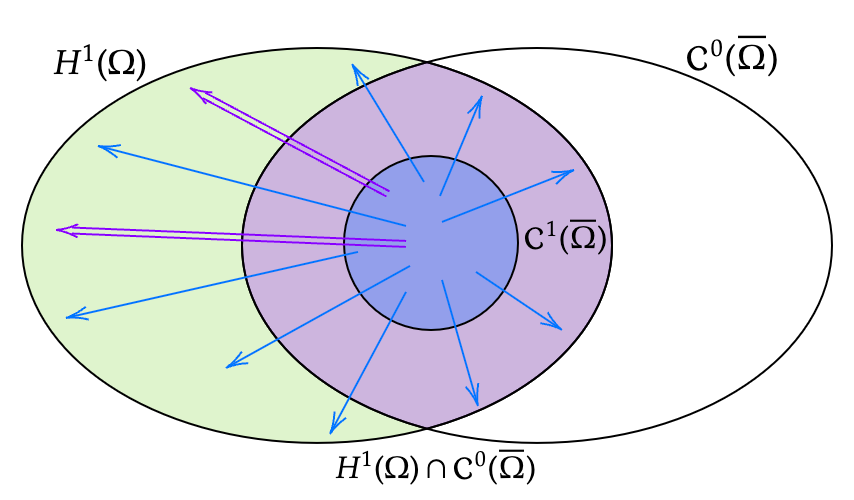
\includegraphics[width=0.9\linewidth]{images/density}\ \ }
\end{Figure}

Before doing so, we need the following: assume $\partial\Omega\in\Cc^\infty$, for every $x_0\in\partial\Omega$ we define $H^s(U_{x_0})$ where $U_{x_0}\subset\RR^{n-1}$ in the sense of local charts, so we found the meaning of $H^s(\partial\Omega)$.

\rule{0.31\textwidth}{0.2pt}
\smallskip

\textbf{Thm.} Let $\Omega\subset\RR^n$ open bdd with $\Cc^\infty$ boundary, and $k\in\NN$. Then, $\exists\,!$ lin. cont. surj. operator 
\begin{gather*}
\gamma_{_0}:H^1(\Omega)\to H^{1/2}(\partial\Omega)\quad\text{such that} \\
\gamma_{_0} u=u\big|_{\partial\Omega}\quad\forall\, u\in\Cc^0(\overline{\Omega})\big(\cap H^1(\Omega)\text{ obv}\big)
\end{gather*}
Moreover, $\exists$ lin. cont. operator 
\begin{gather*}
\Rc:H^{1/2}(\partial\Omega)\to H^1(\Omega)\quad\text{such that} \\
\gamma_{_0}(\Rc g)=g\qquad\forall\, g\in H^{1/2}(\partial\Omega)
\end{gather*}

We call $\gamma_{_0}$ \textbf{trace operator} of order 0, and $\Rc$ \textbf{lift operator} (rilevamento).

\smallskip

\textbf{Rmk:} $\gamma_{_0}$ is unique thanks to the density prop. stated before, $\Rc$ is not unique cause $\gamma_{_0}$ not inv.

\rule{0.31\textwidth}{0.2pt}
\smallskip

\textbf{Thm.} Let $\Omega\subset\RR^n$ open bdd with $\Cc^\infty$ boundary, and $k\in\NN$. Then, $\exists\,!$ $k$ lin. cont. surj. operators $\gamma_{_0},\dots,\gamma_{k-1}$ defined as
\begin{gather*}
\gamma_j:H^k(\Omega)\to H^{k-j-1/2}(\partial\Omega)\quad\forall\,j=0:k-1\\
\text{s.t.}\qquad
\gamma_j u=\frac{\partial^j u}{\partial\nu^j} \bigg|_{\partial\Omega}\qquad\forall\, u\in \Cc^0(\overline{\Omega})
\end{gather*}

We call $\gamma_j$ \textbf{trace operator} of order $j$.

\rule{0.31\textwidth}{0.2pt}
\smallskip

Finally, we can give a characterization of $H^k_0$:

\smallskip

\textbf{Thm.} Let $\Omega\subset\RR^n$ open bdd with $\Cc^\infty$ boundary, $u\in H^k(\Omega)$, with $k\in\NN$. Then:
\begin{equation*}
u\in H^k_0(\Omega) \quad\Longleftrightarrow\quad \gamma_j=0\quad\forall\,j=0:k-1
\end{equation*}

In other words: $H^k_0(\Omega)=\bigcup_j\text{ker}_{\gamma_j}\,.$

\rule{0.31\textwidth}{0.2pt}

% =================================================

\subsection{\texorpdfstring{\color{red}Embedding Thms in \texorpdfstring{$H^k,\ k\in\NN,$}{C} in dim. \texorpdfstring{$n\geq 2$}{C}}{}}

% =================================================

\textbf{Thm (Sobolev).} $\Omega\subset \RR^n$ open with $\partial\Omega\in\text{Lip}$ (or $\Omega=\RR^n$). Then:
\begin{align*}
n=2k\ \leadsto\ &H^k(\Omega)\subset L^p(\Omega)\quad \forall p\in [2,\infty) \\
n>2k\ \leadsto\ &H^k(\Omega)\subset L^p(\Omega)\quad \forall p\in [2,2^*] \\
\begin{array}{c}
\exists\, m\in\NN\text{ s.t.}\\
n<2(k-m)   
\end{array}& 
\leadsto\ H^k(\Omega)\subset \Cc^m(\overline{\Omega})\cap L^\infty(\Omega)\qquad
\end{align*}
where $2^*=\nicefrac{2n}{n-2k}$ is the critical exponent.

\smallskip

\textbf{Rmk:} also for $H^k_0$ without assumptions on $\partial\Omega$.

\rule{0.31\textwidth}{0.2pt}
\smallskip

\textbf{Thm (Sobolev, Rellich, Gagliardo, Nirenberg).} $\Omega\subset \RR^n$ bdd open with $\partial\Omega\in\text{Lip}$.
\begin{align*}
n=2k\ \leadsto\ &H^k(\Omega)\subset\subset L^p(\Omega)\quad \forall p\in [1,\infty) \\
n\geq 2k\ \leadsto\ &H^k(\Omega)\subset\subset L^p(\Omega)\quad \forall p\in [1,2^*)
\end{align*}

\smallskip

\textbf{Rmk:} $p=1$ thx to $L^p$-spaces inclusion ($\Omega$ bdd).

\rule{0.31\textwidth}{0.2pt}

% =================================================

\subsection{\texorpdfstring{\color{red}The spaces \texorpdfstring{$H^{-k},\ k\in\NN,$}{C} in dim. \texorpdfstring{$n\geq 2$}{C}}{}}

% =================================================

$H^{-s}(\Omega):=\left[ H^s_0(\Omega) \right]'$, $H^{-s}(\partial\Omega):=\left[ H^s(\partial\Omega) \right]'$

\rule{0.31\textwidth}{0.2pt}
\smallskip

Let $u:\Omega\subset\RR^n\to\RR^n$.

\smallskip

\textbf{Def.} $\mathbf{E}(\Omega)=\left\{ u\in \mathbf{L}^2(\Omega);\, \nabla\!\!\cdot\! u \in L^2(\Omega) \right\}\equiv \mathbf{L}^2_{\text{div}}$ in the sense of distributions, i.e.
\begin{equation*}
\int_\Omega u\cdot \nabla\varphi=-\int_\Omega (\nabla\cdot u)\, \varphi\quad\forall\,\varphi\in\Dc(\Omega)
\end{equation*}

\smallskip

\textbf{Rmk:} if $n=1$ then $H^1(\Omega)\equiv E(\Omega)$.

\rule{0.31\textwidth}{0.2pt}
\smallskip

\textbf{Thm.} Let $\Omega\subset\RR^n$ open bdd with $\partial\Omega\in\Lip$. Then, $\exists\,!$ lin. cont. surj. operator 
\begin{gather*}
\gamma_{_\nu}:\Ev(\Omega)\to H^{\text{-}1/2}(\partial\Omega)\quad\text{such that} \\
\gamma_{_\nu} u=u\cdot\nu\qquad\forall\, u\in\left[\Cc^0(\overline{\Omega})\right]^n
\end{gather*}

We call $\gamma_{_\nu}$ \textbf{normal trace operator}.

\rule{0.31\textwidth}{0.2pt}
\smallskip

\textbf{Thm (Generalized Gauss-Green formula).} Let $\Omega\subset\RR^n$ open bdd with $\partial\Omega\in\Lip$. Then:
\begin{equation*}
\int_\Omega\!\! u\cdot\nabla\varphi+\int_\Omega\!\varphi\,\Div u={}_{_{H^{\nicefrac{\text{-}1}{2}}}}\!\!\sca{\gamma_{_\nu} u,\,\gamma_{_0}\varphi}\!\!{}_{_{H^{\nicefrac{1}{2}}}}
\end{equation*}

$\forall\, u\in\Ev(\Omega),\ \varphi\in H^1(\Omega)$.

\rule{0.31\textwidth}{0.2pt}
\smallskip

We'll apply this to $u:\Omega\to\RR$ (e.g. Neumann problem) where $u\in H^1$ with $\Delta u\in L^2$. Indeed, $\nabla u \in \mathbf{L^2}$ with $\nabla\!\cdot\!\nabla u \in L^2$, i.e. $\nabla u \in \mathbf{E}$. Then $\exists\, !$
\begin{equation*}
\gamma_{_\nu} \nabla u=\nabla u \cdot \nu = \frac{\partial u}{\partial \nu} 
\end{equation*}
and the Gauss-Green formula becomes
\begin{equation*}
\int_\Omega\!- \Delta u\ v=\int_\Omega \nabla\! u\,\nabla\! v -\sca{\frac{\partial u}{\partial \nu}, \gamma_{_0} v}\quad\forall\, v\in H^1
\end{equation*}

\rule{0.31\textwidth}{1pt}










